\documentclass[12pt,a4paper]{report}
\usepackage[utf8]{inputenc}
\usepackage[french]{babel}
\usepackage[T1]{fontenc}
\usepackage{amsmath}
\usepackage{amsfonts}
\usepackage{amssymb}
\usepackage{makeidx}
\usepackage{graphicx}
\usepackage[left=2cm,right=2cm,top=2cm,bottom=2cm]{geometry}
\author{Musiques et Recherches}
\title{Configuration salle : Studio 1 \\ Adresse :  Place Flagey}
 \begin{document}
\maketitle
\chapter*{Vue d'ensemble}
 \begin{center}
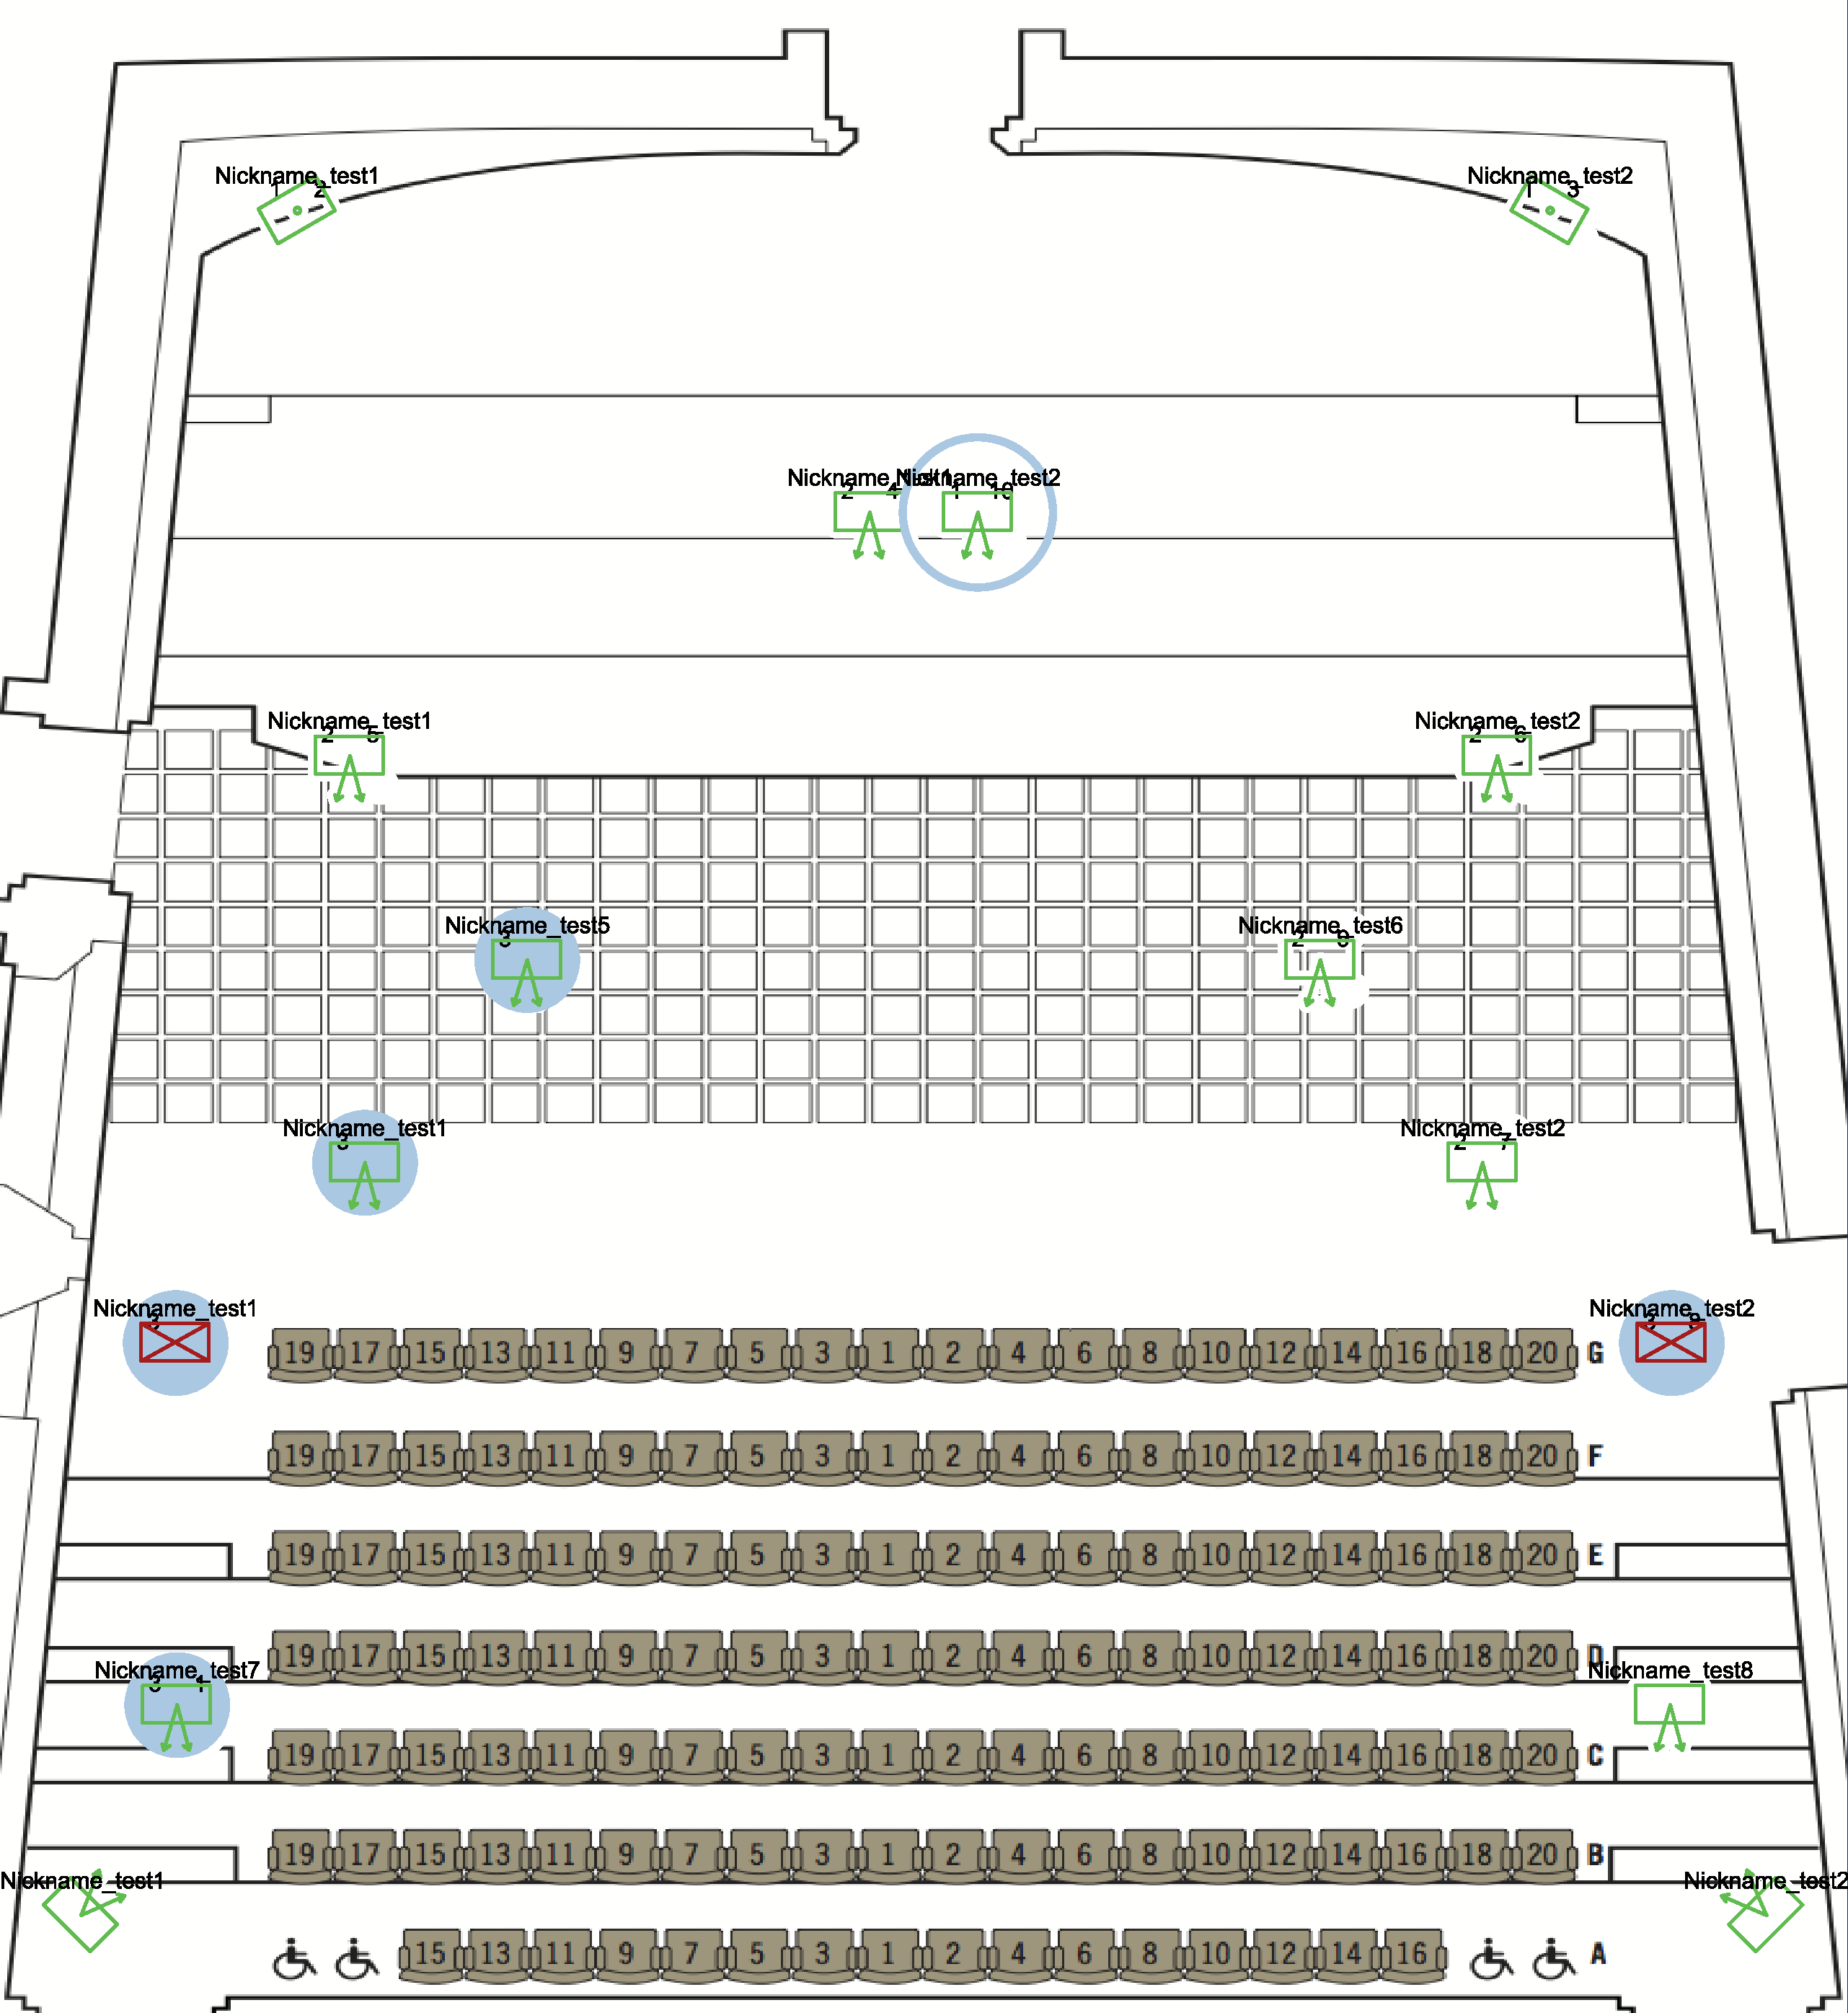
\includegraphics[height=20cm]{data/planSalle123.pdf}
\end{center}
 \chapter*{Association pistes audios - Curseur - Sortie}
 \begin{center}
 \begin{tabular}{|c|c|c|}
 \hline 
 Piste Audio & Curseur & Sortie MADI \\ 
\hline 
2 & 1 & 9 \\ 
 \hline 
1 & 2 & 10 \\ 
 \hline 
3 & 1 & 1 \\ 
 \hline 
4 & 2 & 4 \\ 
 \hline 
5 & 3 & 5 \\ 
 \hline 
5 & 4 & 6 \\ 
 \hline 
4 & 4 & 7 \\ 
 \hline 
3 & 3 & 8 \\ 
 \hline 
1 & 2 & 2 \\ 
 \hline 
2 & 1 & 3 \\ 
 \hline 

 \end{tabular}  

 \end{center}
 \chapter*{Association MADI - Ampli - haut-parleurs}
 \begin{center}
 \begin{tabular}{|c|c|c|}
 \hline 
 sortie MADI & Ampli & Haut-parleur \\ 
\hline 
9 & TODO & Altec 50 - Voix de Théatre 1 \\ 
 \hline 
10 & TODO & Altec 50 - Voix de Théatre 2 \\ 
 \hline 
1 & TODO & JBL 4435 1 \\ 
 \hline 
4 & TODO & JBL 4435 2 \\ 
 \hline 
5 & TODO & Audiotools - 1 \\ 
 \hline 
6 & TODO & Audiotools - 2 \\ 
 \hline 
7 & TODO & Audiotools - 3 \\ 
 \hline 
8 & TODO & Audiotools - 4 \\ 
 \hline 
2 & TODO & Audiotools - 5 \\ 
 \hline 
3 & TODO & Audiotools - 6 \\ 
 \hline 

 \end{tabular}  

 \end{center}
 \end{document}  

